\subsection{Interrelación Reunión - Pregunta Oficial}

   \begin{description}
      \item[Definición] En esta interrelación se deja constancia de que una
      reunión puede estar compuesta por varias preguntas oficiales.

      \item[Características] La interrelación presenta las siguientes
                             características:

         \begin{itemize}
            \item \textbf{Nombre:} R-PO
            \item \textbf{Tipo de la interrelación:} Fuerte.
            \item \textbf{Cardinalidad de la interrelación:} N:M
                  \begin{itemize}
                     \item Reunión: compuesta\_por (0,n)
                     \item Pregunta Oficial: aparece\_en (0,n)
                  \end{itemize}
            \item \textbf{Número de atributos:} Uno: respuesta.
         \end{itemize}

      \item[Diagrama] La figura \ref{diagramaR-PO} muestra el diagrama de la
                      interrelación.

      \item \begin{figure}[!ht]
            \begin{center}
            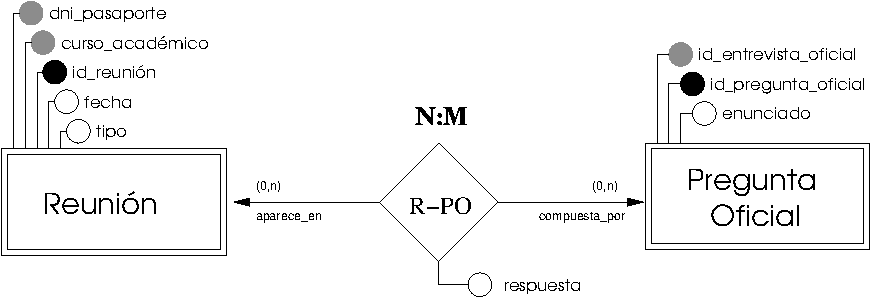
\includegraphics[]{07.Modelo_Entidad-Interrelacion/7.3.Analisis_Interrelaciones/diagramas/R-PO.pdf}
            \caption{Diagrama de la interrelación R-PO.}
            \label{diagramaR-PO}
            \end{center}
         \end{figure}

      \item[Descripción de los atributos] La interrelación presenta el
      siguiente atributo:

       \begin{itemize}
        \item \textbf{respuesta}
          \begin{itemize}
            \item \textbf{Definición:} Establece la contestación del alumno a la
            pregunta realizada.
            \item \textbf{Dominio:} Conjunto de caracteres alfanuméricos.
            \item \textbf{Carácter:} Obligatorio.
            \item \textbf{Ejemplo práctico:} Antiguo alumno.
            \item \textbf{Información adicional:} El dato lo introduce el
            usuario alumno al contestar a la pregunta realizada.
         \end{itemize}
       \end{itemize}

      \item[Ejemplo práctico del tipo de interrelación]

      \item \begin{center}
            \begin{tabular}{ | r r | }
            \hline
            \multicolumn{2}{ | c | }{\textbf{Tipo de interrelación R-PO}} \\
            \hline
            \textbf{Reunión} & \\
            dni\_pasaporte & 98765432Z \\
            curso\_académico & 2008 \\
            id\_reunión & 121 \\
            fecha & 01/01/2009 \\
            tipo & Individual \\
            \hline
            \textbf{Pregunta Oficial} & \\
            id\_entrevista\_oficial & 24 \\
            id\_pregunta\_oficial & 55 \\
            enunciado & ¿Quién le ha informado de esta carrera? \\
            \hline
            \textbf{Atributos} & \\
            respuesta & Antiguo alumno \\
            \hline
            \end{tabular}
         \end{center}
   \end{description}
